\documentclass{article}

\usepackage[utf8]{inputenc} %Only required if not using XeLatex
\usepackage[T1]{fontenc}
\usepackage[final]{microtype}
\usepackage{bm} %Bold font for math equations

\usepackage{verbatim} %For word count
\newcommand{\detailtexcount}[1]{\immediate\write18{texcount -merge -sum -nobib  #1.tex output.bbl > #1.wcdetail}\verbatiminput{#1.wcdetail}}

\usepackage{helvet} %Set font type (helvetica)
\renewcommand{\familydefault}{phv} %Set helvetica as default font

\usepackage[a4paper, margin=25mm]{geometry} %Setting document size and margin width

\usepackage{enumitem} %Custom list
\newlist{arrowlist}{itemize}{1} %Define custom list name
\setlist[arrowlist]{label=$\rightarrow$} %Define arrow for custom list label

\usepackage[url=false, doi=false, isbn=false, bibstyle=ieee, citestyle=numeric-comp]{biblatex} %Set bibliography style
\addbibresource{Lit_rev.bib} %Imports .bib file

\usepackage{graphicx} %Required for graphics and figures
\graphicspath{ {./Fig/} }
\usepackage[export]{adjustbox} %Used for adjusting image box
\usepackage{caption} %For caption customizations
\usepackage{subcaption}

\title{\textbf{Literature Review \\and \\Lay Summary}}
\author{Jasper Ng}
\date{May 2025}

\begin{document}

\maketitle

%TC:ignore
\noindent{\textbf{\Large Uncertainty Quantification of Plasma Filament in the Tokamak \\Scrape-off Layer}}

\begin{figure}[h]
    \centering
    \begin{subfigure}[c]{0.45\linewidth}
        \centering
        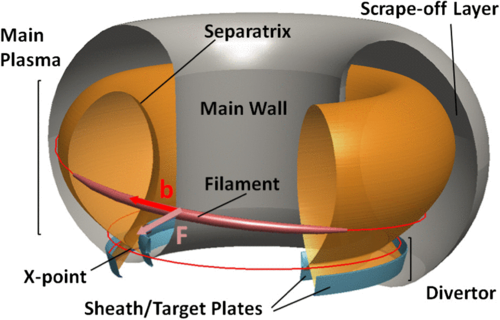
\includegraphics[width=0.9\linewidth]{Fig1_plasma_filament.png}
        \normalsize{\caption{Example of a plasma filament along a magnetic field line in the SOL \cite{carralero_experimental_2015}}}
        \label{fig:fig1}
    \end{subfigure}
    \hspace{0.05\linewidth}
    \begin{subfigure}[c]{0.45\linewidth}
        \centering
        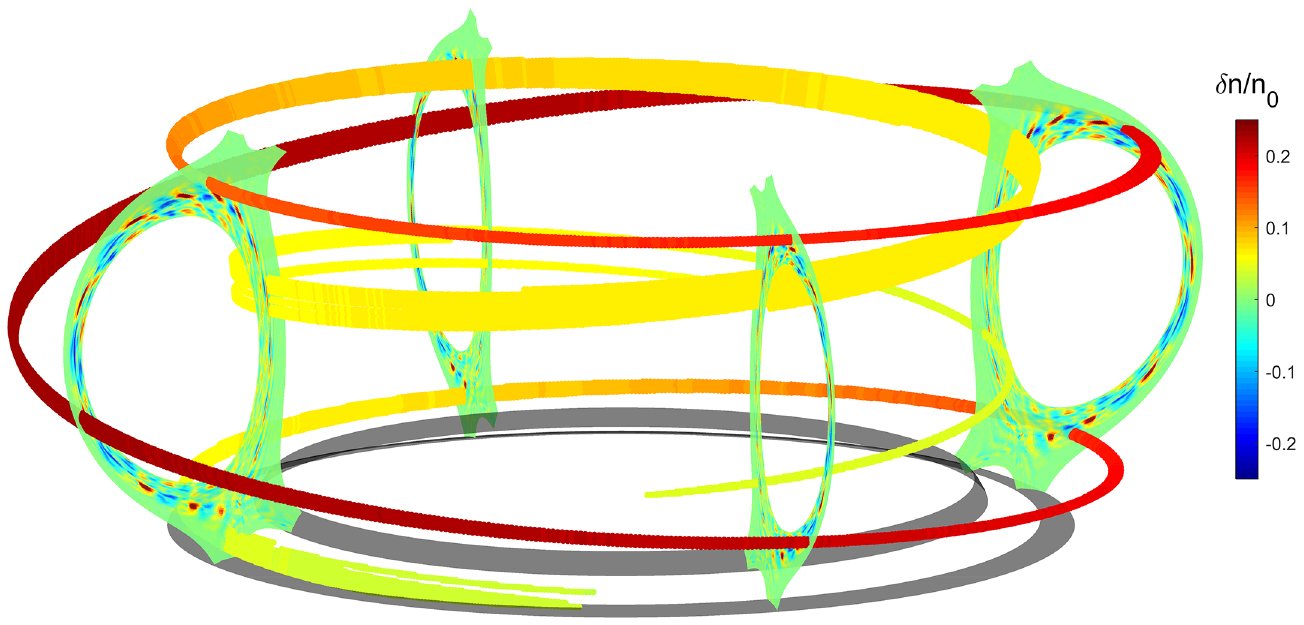
\includegraphics[width=0.9\linewidth]{Fig2_blob_movement.png}
        \normalsize{\caption{Density and movement of a blob with average density on the 4 poloidal planes \cite{nespoli_3d_2019}}}
        \label{fig:fig2}
    \end{subfigure}
    \normalsize{\caption{Simulations of a blob in tokamak plasmas}}
\end{figure}

\section*{Plan}
\subsection*{Plasma Filament (Blobs)}
\begin{itemize}
    \item What are plasma filaments
    \begin{itemize}
        \item Found in various magnetic fusion device, occurring in various regimes such as L and H mode \cite{boedo_transport_2003} and ELM mode \cite{ben_ayed_inter-elm_2009}
        \item Important as it affects particle transport and heat flux in SOL, and directly impacts durability and lifetime of plasma facing materials \cite{carralero_experimental_2015, krasheninnikov_recent_2008}
        \item Blob formation \cite{krasheninnikov_recent_2008}:
        \begin{enumerate}
            \item Turbulent processes (or MHD instabilities) causes plasma peel off at outmost layer (curvature and $\nabla$B induced F$\times$B drifts)
            \item Plasma polarization due to gravity drift
            \item Vertical charge separation induces E field ($\perp$ to toroidal B field)
            \item Diamagnetic divergence gives current source in direction $\perp$ to drifts and hence circuit must be closed (through parallel or polarization current) \cite{omotani_effects_2015}
            \begin{itemize}
                \item Polarisation current: leads to inertial evolution and blob pushed by $J\times B$ force
                \item Parallel current: leads to sheath dissipation and current induces potential due to sheath resistivity, blob pushed by $E\times B$ force from potential
            \end{itemize}
        \end{enumerate}
        \item Large amount of 2D and 3D simulations \cite{omotani_effects_2015, easy_three_2014, nespoli_3d_2019, garcia_mechanism_2005, shanahan_fluid_2018} done to model blob structure and dynamic of blob to understand filament transport  
    \end{itemize}
    \item Blob parameters and equations for 2D simulation (specifically blob2d in BOUT++) \cite{omotani_effects_2015}
    \begin{itemize}
        \item Density n
         \begin{itemize}
            \item $L_{\parallel}$ is magnitude, $\phi$ is elctrostatic potential, $\bm{\hat{b}}$ is the unit vector in direction of magnetic field ($\bm{\hat{b}}=\bm{B}/B$), A is amplitude of filament, $\epsilon$ is the ratio of length of axes of the ellipse, $\alpha$ is tilted angle to x direction
        \end{itemize}
        \begin{arrowlist}
            \item $\frac{dn}{dt}=\bm{\hat{b}\cdot g}\times \left(n\nabla\phi-\nabla n\right)+\frac{n\left(1-e^{-\phi}\right)}{L_{\parallel}}+\mu_n\nabla^2_{\perp}n$
            \item $n\left(t=0\right)=n_0\left(1+A\exp{\left(-\frac{{{x'}^2/\epsilon}\,+\,{\epsilon {z'}^2}}{\delta^2}\right)}\right)$
            \item $x'=x\,cos\,\alpha\,+\,z\,sin\,\alpha$
            \item $z'=z\,cos\,\alpha\,-\,x\,sin\,\alpha$
        \end{arrowlist}
        \item Vorticity $\Omega$
            \begin{itemize}
            \item $V_{E\times B}$ is the $E\times B$ velocity
            \end{itemize}
        \begin{arrowlist}
            \item $\frac{d\Omega}{dt}=-\frac{1}{2}\bm{\hat{b}\cdot}\nabla V^2_{E\times B}\times \nabla n-\bm{\hat{b}\cdot g}\times\nabla n+\frac{n\left(1-e^{-\phi}\right)}{L_{\parallel}}+\mu_i\nabla^2_{\perp}\Omega$
            \item $\Omega=\nabla\cdot\left(n\nabla_{\perp}\phi\right)$
        \end{arrowlist}
        \item Filament size $\delta_x$,$\delta_z$
            \begin{itemize}
            \item $\delta$ is the geometric mean of the lengths of the axes
            \end{itemize}
            \begin{arrowlist}
            \item $\delta_x=\delta\sqrt{\frac{\epsilon}{\left(cos^2\alpha\,+\,\epsilon^2sin^2\alpha\right)}}$
            \item $\delta_z=\delta\sqrt{\frac{\epsilon}{\left(\epsilon^2cos^2\alpha\,+\,sin^2\alpha\right)}}$
        \end{arrowlist}
        \item Maximum velocity $V_f$
        \begin{itemize}
            \item Velocity scales with filament size and depends on regime
            \item $\delta_x$ is lengthscale in x-direction. $R_c$ is radius of curvature of magnetic field (major radius), $\beta$ is constant
        \end{itemize}
        \begin{arrowlist}
            \item Polarisation current (narrow filament): $V_f\sim\sqrt{gA\delta_x}$ ($g=\frac{1}{R_c}$)
            \item Parallel current (wide filament): $V_f\sim \frac{L_{\parallel}g}{\delta^2_z}\frac{A}{1+\beta A}$
        \end{arrowlist}
    \end{itemize}
\end{itemize}

\subsection*{Uncertainty Quantification}
    \subsubsection*{Surrogate Model}
    \begin{itemize}
        \item Used to approximate mathematical models and maps inputs to outputs without knowing the relationship between design and output variables \cite{williams_novel_2021}
        \item Gaussian Processes
        \begin{itemize}
            \item What are Gaussian processes \cite{hornsby_gaussian_2024}
            \begin{itemize}    
                \item Machine learning method based on gaussian distributions
                \item For each pairs of variables, compares the correlation between the variables (covariance)
                \item Kernels are functions chosen to assume the distribution, used to generate a covariance matrix and that test points (variables) that are close should yield similar results (small covariance) \cite{duvenaud_automatic_2014}
                \item Training data are then added to covariance matrix for evaluation, and are points kernel functions must pass through and posterior distribution is found (most likely result)
                \item Kernels can be combined to yield better approximations \cite{duvenaud_automatic_2014}
            \end{itemize}
        \end{itemize}
    \end{itemize}
    \subsubsection*{Sensitivity Analysis \cite{wirthl_global_2023} } 
    \begin{itemize}
        \item Uncertainty of model output found using model inputs, including input parameters, boundary and initial conditions etc.
        \item Can help to identify the significance of input parameters
        \item Sobol Method
        \begin{itemize}
            \item Variance based method
            \item Requires large amount of model evaluations
            \item Sobol indices are calculated for each variable, with higher value being more influential
            \item Total-order Sobol indexis then calculated to determine if a parameter is non-influential and can be fixed if determined non-influential
        \end{itemize}
    \end{itemize}
\pagebreak
%TC:endignore

%TC:ignore
\noindent{\textbf{\Large Uncertainty Quantification of Plasma Filament in the Tokamak \\Scrape-off Layer}}
%TC:endignore
\section*{Literature Review}
\subsection*{Overview}
Plasma filaments or blobs are coherent plasma structures that form from perturbations in the Scrape-off Layer (SOL) that transport heat and material across the magnetic field lines \cite{dippolito_convective_2011, hoare_dynamics_2019}. It is useful to perform simulations on the filament as it could help to review particle and heat transport of the plasma at the SOL, as well as the impact on the durability and lifetime of plasma facing materials and vessel walls \cite{carralero_experimental_2015, krasheninnikov_recent_2008}. In order to aid simulation, it would be useful to quantify the importance of each of the parameters that govern the properties of the blob.

Uncertainty quantification is a framework that could model the uncertainties of the governing model parameters and the effect it has on the overall system \cite{sudret_surrogate_2017}. Using a surrogate model such as Gaussian processes, a sensitivity analysis can be performed on the parameters of the governing equations relating to the properties of the plasma filaments.

Through the use of uncertainty quantification, the parameters of the equations that govern plasma filament property could be analysed whilst avoiding being computationally expensive. 
\subsection*{Plasma Filament}
Plasma filaments are a common feature among magnetic fusion devices in different operating modes, appearing in devices such as tokamaks and stellarators and in operating modes including L-mode, H-mode and edge localised modes (ELMs) \cite{ben_ayed_inter-elm_2009, killer_plasma_2020, boedo_transport_2003}. The importance of this feature was due to the discovery of plasma recycling within the main chamber of the reactor, and instead of the fusion plasma flowing to the divertor it was flowing into the chamber walls \cite{krasheninnikov_recent_2008,dippolito_convective_2011}.

The mechanism for blob formation was proposed by Krashennikov \textit{et al.} \cite{krasheninnikov_recent_2008, krasheninnikov_scrape_2001}. At first, the plasma would be separated and formed at the outmost layer of the SOL due to turbulent processes. Plasma polarization of the separated plasma would then occur due to particle drift effects within the vessel, such as the curvature drift and the $\bm{\nabla B}$ drift. The vertical charge separation then induces an $\bm{E}$ field in the perpendicular direction to the toroidal direction, leading to an $\bm{E}\times\bm{B}$ force on the plasma radially outward. An alternative mechanism of the current source was proposed by Omotani \textit{et al.} that a current source was due to the diamagnetic current drift in the plasma instead of the particle drifts. To maintain quasineutrality in the plasma, the circuit would be closed through polarisation current or parallel current configuration.

As reviewed by \cite{dippolito_convective_2011} there are a large amount of simulations in 2D and 3D simulations done to understand blob dynamics with different closure schemes for the 2D model that explains the motion and properties of the blob. The most common is the sheath limited model assuming that the circuit is closed through the sh



\nocite{*}
\printbibliography[title={References}]

%TC:ignore
\detailtexcount{Lit_rev}
%TC:endignore

\end{document}

